%%%%%%%%%%%%%%%%%%%%%%%%%%%%%%%%%%%%%%%%%%%%%%%%%%%%%%%%%%%%%%%%%%%%%%%%%%%%%
%%%
%%% File: thesis.tex, version 1.9, May 2015
%%%
%%% =============================================
%%% This file contains a template that can be used with the package
%%% cs.sty and LaTeX2e to produce a thesis that meets the requirements
%%% of the Computer Science Department from the Technical University of Cluj-Napoca
%%%%%%%%%%%%%%%%%%%%%%%%%%%%%%%%%%%%%%%%%%%%%%%%%%%%%%%%%%%%%%%%%%%%%%%%%%%%%

\documentclass[12pt,a4paper,twoside]{report} 

\usepackage{cs}              
\usepackage{times}
\usepackage{float}
\usepackage[caption = false]{subfig}
\usepackage{graphicx}
\usepackage{latexsym}
\usepackage{amsmath,amsbsy}
\usepackage{amssymb}
\usepackage[matrix,arrow]{xy}
\usepackage[T1]{fontenc}
\usepackage{ae,aecompl}
%\usepackage{shortcut} %definitii pentru diacritice; 
\usepackage{amstext}
\usepackage{graphics}
\usepackage[T1]{fontenc}
\usepackage{ae,aecompl}
\usepackage{algorithm}
%\usepackage{algorithmic}
\usepackage{color}
\usepackage{color}

% \mastersthesis
\diplomathesis
% \leftchapter
\centerchapter
% \rightchapter
\singlespace
% \oneandhalfspace
% \doublespace

\renewcommand{\thesisauthor}{Firstname LASTNAME}    %% Your name.
\renewcommand{\thesismonth}{June}     %% Your month of graduation.
\renewcommand{\thesisyear}{2015}      %% Your year of graduation.
\renewcommand{\thesistitle}{LICENSE THESIS TITLE} 
\renewcommand{\thesissupervisor}{scientific title Firstname LASTNAME}
\newcommand{\department}{\bf FACULTY OF AUTOMATION AND COMPUTER SCIENCE\\
COMPUTER SCIENCE DEPARTMENT}
\newcommand{\thesis}{LUCRARE DE LICEN'T'A}
\newcommand{\utcnlogo}{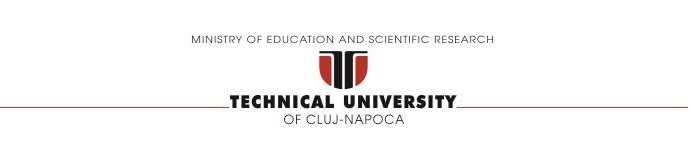
\includegraphics[width=15cm]{img/tucn.jpg}}

\newcommand{\uline}[1]{\rule[0pt]{#1}{0.4pt}}
%\renewcommand{\thesisdedication}{P\u{a}rin\c{t}ilor mei}

\begin{document}
%\frontmatter
%\pagestyle{headings}

\newenvironment{definition}[1][Defini\c{t}ie.]{\begin{trivlist}
\item[\hskip \labelsep {\bfseries #1}]}{\end{trivlist}}



%\thesistitle                    %% Generate the title page.
%\authordeclarationpage                %% Generate the declaration page.

\pagenumbering{arabic}
\setcounter{page}{4}



\begin{center}
\utcnlogo

\department

\vspace{4cm}

{\bf \thesistitle} %LICENSE THESIS TITLE}

\vspace{1.5cm}

LICENSE THESIS

\vspace{6cm}

Graduate: {\bf Firstname LASTNAME} 

Supervisor: {\bf \thesissupervisor}

\vspace{3cm}
{\bf \thesisyear}
\end{center}

\thispagestyle{empty}
\newpage

\begin{center}
\utcnlogo

\department

\end{center}
\vspace{0.5cm}

%\begin{small}
\begin{tabular}{p{7cm}p{8cm}}
 %\hspace{-1cm}& APPROVED,\\
 \hspace{-1cm}DEAN, & HEAD OF DEPARTMENT,\\
\hspace{-1cm}{\bf Prof. dr. eng. Liviu MICLEA} & {\bf Prof. dr. eng. Rodica POTOLEA}\\  
\end{tabular}
 
\vspace{2cm}

\begin{center}
Graduate: {\bf \thesisauthor}

\vspace{1cm}

{\bf \thesistitle}
\end{center}

\vspace{1cm}

\begin{enumerate}
 \item {\bf Project proposal:} {\it Short description of the license thesis and initial data}
\item {\bf Project contents:} {\it (enumerate the main component parts) Presentation page, advisor's evaluation, title of chapter 1, title of chapter 2, ..., title of chapter n, bibliography, appendices.}
\item {\bf Place of documentation:} {\it Example}: Technical University of Cluj-Napoca, Computer Science Department
\item {\bf Consultants:}
\item {\bf Date of issue of the proposal:} November 1, 2014
\item {\bf Date of  delivery:} June 18, 2015 {\it (the date when the document is submitted)}
  \end{enumerate}
\vspace{1.2cm}

\hspace{6cm} Graduate: \uline{6cm} 

\vspace{0.5cm}
\hspace{6cm} Supervisor: \uline{6cm} 
%\end{small}

\thispagestyle{empty}


\newpage
$ $
%\begin{center}
%\utcnlogo

%\department
%\end{center}

\thispagestyle{empty}
\newpage

\begin{center}
\utcnlogo

\department
\end{center}

\vspace{0.5cm}

\begin{center}
{\bf
Declara\c{t}ie pe proprie r\u{a}spundere privind\\ 
autenticitatea lucr\u{a}rii de licen\c{t}\u{a}}
\end{center}
\vspace{1cm}



Subsemnatul(a) \\
\uline{14.8cm}, 
legitimat(\u{a}) cu \uline{4cm} seria \uline{3cm} nr. \uline{4cm}\\
CNP \uline{9cm}, autorul lucr\u{a}rii \uline{2.8cm}\\
\uline{16cm}\\
\uline{16cm}\\
elaborat\u{a} \^{\i}n vederea sus\c{t}inerii examenului de finalizare a studiilor de licen\c{t}\u{a} la Facultatea de Automatic\u{a} \c{s}i Calculatoare, Specializarea \uline{7cm} din cadrul Universit\u{a}\c{t}ii Tehnice din Cluj-Napoca, sesiunea \uline{4cm} a anului universitar \uline{3cm}, declar pe proprie r\u{a}spundere, c\u{a} aceast\u{a} lucrare este rezultatul propriei activit\u{a}\c{t}i intelectuale, pe baza cercet\u{a}rilor mele \c{s}i pe baza informa\c{t}iilor ob\c{t}inute din surse care au fost citate, \^{\i}n textul lucr\u{a}rii \c{s}i \^{\i}n bibliografie.

Declar, c\u{a} aceast\u{a} lucrare nu con\c{t}ine por\c{t}iuni plagiate, iar sursele bibliografice au fost folosite cu 
respectarea legisla\c{t}iei rom\^{a}ne \c{s}i a conven\c{t}iilor interna\c{t}ionale privind drepturile de autor.

Declar, de asemenea, c\u{a} aceast\u{a} lucrare nu a mai fost prezentat\u{a} \^{\i}n fa\c{t}a unei alte comisii de examen de licen\c{t}\u{a}.

\^{I}n cazul constat\u{a}rii ulterioare a unor declara\c{t}ii false, voi suporta sanc\c{t}iunile administrative, respectiv, \emph{anularea examenului de licen\c{t}\u{a}}.

\vspace{1.5cm}

Data \hspace{8cm} Nume, Prenume

\vspace{0.5cm}

\uline{3cm} \hspace{5cm} \uline{5cm}

\vspace{1cm}
\hspace{9.4cm}Semn\u{a}tura

\thispagestyle{empty}

\newpage


%\listoftables
%\listoffigures

%\clearpage 
%\newpage

%\begin{comment}
{\color{red}{\bf De citit \^{\i}nainte} (aceast\u{a} pagin\u{a} se va elimina din versiunea final\u{a})}:
\begin{enumerate}
 \item Cele trei pagini anterioare (foaie de cap\u{a}t, foaie sumar, declara\c{t}ie) se vor lista pe foi separate (nu fa\c{t}\u{a}-verso), fiind incluse \^{\i}n lucrarea listat\u{a}. 
 Foaia de sumar (a doua) necesit\u{a} semn\u{a}tura absolventului, respectiv a coordonatorului.
 Pe declara\c{t}ie se trece data c\^{a}nd se pred\u{a} lucrarea la secretarii de comisie.
 \item Pe foaia de cap\u{a}t, se va trece corect titulatura cadrului didactic \^{\i}ndrum\u{a}tor, \^{\i}n englez\u{a} (consulta\c{t}i pagina de unde a\c{t}i desc\u{a}rcat acest document pentru lista cadrelor didactice cu titulaturile lor).
 \item Documentul curent {\bf nu} a fost creat \^{\i}n MS Office. E posibil sa fie mici diferen\c{t}e de formatare. 
\item Cuprinsul \^{\i}ncepe pe pagina nou\u{a}, impar\u{a} (dac\u{a} se face listare fa\c{t}\u{a}-verso), prima pagin\u{a} din capitolul \emph{Introducere} tot a\c{s}a, fiind numerotat\u{a} cu 1. % Pentru actualizarea cuprinsului, click dreapta pe cuprins (zona cuprinsului va apare cu gri), Update field-$>$Update entire table.
\item E recomandat s\u{a} vizualiza\c{t}i acest document \c{s}i \^{\i}n timpul edit\u{a}rii lucr\u{a}rii. % după ce activaţi vizualizarea simbolurilor ascunse de formatare (apăsaţi simbolul  din Home/Paragraph).
\item Fiecare capitol \^{\i}ncepe pe pagin\u{a} nou\u{a}. % datorită simbolului ascuns Section Break (Next Page) care este deja introdus la capitolul precedent. Dacă ştergeţi din greşeală simbolul, se reintroduce (Page Layout -> Breaks).
\item Folosi\c{t}i stilurile predefinite (Headings, Figure, Table, Normal, etc.)
\item Marginile la pagini nu se modific\u{a}.
\item Respecta\c{t}i restul instruc\c{t}iunilor din fiecare capitol.
\end{enumerate}
 
%\end{comment}

\newpage

\tableofcontents
\newpage



\chapter{Introduction - Project Context}
\pagestyle{headings}
{\color{red}{must be about 3 pages}}

Optical flow is big area of research form computer vision. It is given by a vector field of velocities which describe the movement of the elements of the projected environment. With a large range of applications, it is a rich source of information. 

The optical flow problem does not originate in computer vision, but in psychology, psychophysics. One of the most influential man in this field is J.J. Gibson. He was the one who stated the problem as "How do we see the world around us?". In his many publications around the 50's, he tries to explain this phenomena and describes some principles that stand at the foundation of modern day approaches.  In his book\cite{gibson1950perception}, Gibson explains how the stimuli are correlated to the perception of motion. 
We perceive the motion in 2D as a projection of the 3D world. This projection is nothing else but the light reflected from the environment, hitting our retina, referred as the optical array. In a analytical context, he defines the movement for a perception. Each element is detected and associated a pair of coordinates. Then each element has a motion descriptor as either a pair of elements or a speed and direction component, in successive moments in time. 

As the nature is the grand engineer, the same model is taken in computer vision for computing the optical flow. The changes in the optical array are stocked in a series of frames. The perceived image is a 2D array of pixels. Each pixel is a element in the movement. An accurate and robust flow estimation implies an approximation for each pixel of the frame. The result will be a vector field indicating the direction and that each pixel takes between frames.
 
This is a old field of study.
Further we will discuss dense flow algorithms. Unlike sparse algorithms that precess only relevant features op the frame sequence, like corners or edges, dense methods compute the flow for each pixel of the image.

 The first algorithms were published in 1980. They are the foundations of modern approaches. Computing a energy function fro the sequence of frames and the flow, and trying to minimize it is the short description for most of the algorithms. For example, the brightness constraint formulated by Horn and Schunk is still the starting point of many algorithms in describing the energy function. Also, the pyramidal implementation of Horn and Schunk's it is also present in modern approaches, solving the large displacement problem. This are some of the fundamental concepts stated by the fathers of optical flow. All this will be further discussed in the next chapters.
  
This core algorithms were for a long time considered the benchmark for other algorithms in dense optical flow. 
In time others researchers brought their contribution to the field of study by small changes in the previous algorithms. Changes vary from particularizing the weight of contribution of each pixel to the computation to adding new terms to the minimization problem, to even rewriting the energy function in a different penalty. 

With decades of small steps to improvement, algorithms today reach a high accuracy, increased with up to 13 times from the original Lucas-Kanade in terms of angular error as can be seen on Middlebury database, and can reach near real time speed.

In the next section this fundamental algorithms will be discussed in detail.

In the next chapter,  \ref{POS} we will discuss what is the optical flow and some examples will be explained. Then we will shortly talk in ensemble about what is its mathematical form, what are the main approaches in finding it. 



\chapter{Project Objectives and Specifications} \label{POS}
{\color{red}{must be about 6 pages}}


Optical field computation is a complex area of study. From the first methods published around 1980, the field advanced trough the decades little by little, up to these days when it can bee computed with high accuracy, and the computation time comes close to real time.


\section{Optical Flow definitions and examples}

The optical flow is defined from a field of vectors $(u,v)$ which define the velocities of the pixels in a image.
Solving the optical flow means finding this $(u,v)$ correspondence between the pixels of 2 consecutive frames.

Let us dfine the optical flow on the example in image \ref{movingDot}. If we have the 2 frames, which are consecutive in time, we observe the white dot in the first frame $(x,y)$. In the second frame it had moved up and to the right, reaching the position $(x+1, y+v)$. Now, The flow is defined by the displacement of this dot. We say that the flow is defined by the vector $(u,v)$. The assumption on which most of the dense models are formulated is that moving pixels do not change their intensity in time. In our example $$I(x,y) = I(x+u, y+v)$$.

Taking an more complex example, \ref{moreflow} the optical field is composed from $m\cdot n$ vectors corresponding to each pixel. This exemplifies the flow between image frames, which are matrices of pixels. The algorithms that compute such a structure for the flow are called dense, unlike sparse methods that compute the flow only for key features of the frames. The flow is formulated in a energy function, based on the brightness  constraint and others, depending on the algorithm. This function should be ideally $0$. A simple (but not very efficient) example of the energy function is $\sum |I(x,y) - I(x+u, y+v)|$. In \ref{moreflow} if we add all the difference between pixels in the first image and their corresponding from the next, we will find that the result is 0.
\begin{figure} \label{movingDot}
\centering
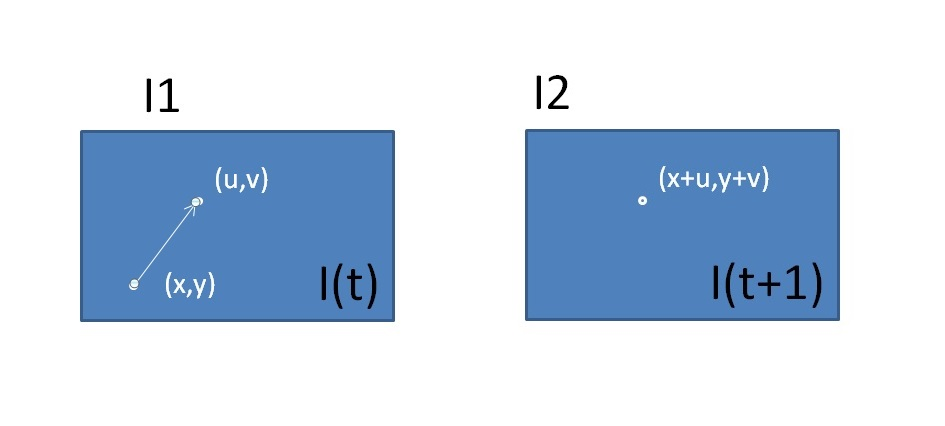
\includegraphics[width = 5in]{img/movingDot} 
	\caption{Moving Dot}
\end{figure}


\begin{figure} \label{moreflow}
	\centering
	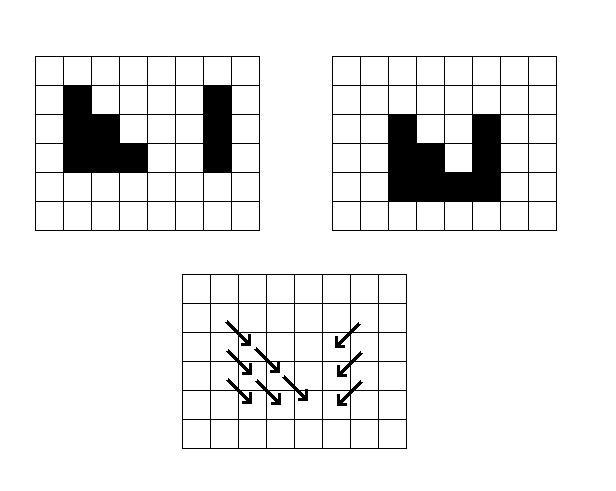
\includegraphics[width = 5in]{img/morefow} 
	\caption{Moving Objects}
\end{figure}

\section{Solving the Optical Flow System}

Solving the system is the expensive part of the algorithm. The solution available is based on the chosen model. The classic formulation are based om a $L^2$ norm. With variational calculus, their derivatives are equated to 0. For this simple solvers are available. Gauss-Seidel and Jacobi iterations are the most handy solution. They are simple, fast, and memory inexpensive. This are classic approaches for the $L^2$ norm. We used them to implement the Horn and Schunk method and they are discussed in the next chapters.

In latest approaches there is a tendency to lose the $L^2$ formulation in favour of the $L^1$. Although it is more computationally expensive to solve then, this formulations are preferred because of it's robustness. Our final implementation is based on such a formulation. 

\section{Project Objectives}


The project has two objectives, one is gathering some research in the field, and the second is implementing our solution with a new minimizing strategy.

With a highly complex mathematical model and a large numbers of approaches, the main scope of this project is to familiarize with the basic concepts and methods of the optical flow computation. The two ground approaches, Horn Schunk and Lucas Kanade were studied, implemented, and will be discussed in detail in the next chapters. Then as a starting point for our algorithm we stareted from Drulea's paper, \cite{drulea2013}, which was studied, implemented and tested. Then a new strategy of minimization was studied, then implemented wit the formulation from the previous algorithm. The results are compared with the starting algorithm and other small modifications are implemented to learn the effect and possible improvements.


\chapter{Bibliographic research}




Optical Flow problem is an old subject in computer vision. The fundamental method for robust optical flow, referenced in over $10000$ articles up to the newest, was published in 1980, by Horn and Schunch ~\cite{HSOpticalFlow}. They define the optical flow as
\begin{quote}
"the distribution of apparent velocities of movement in an image."
\end{quote}
and state the problem as a minimization of a squared penalty function from the brightness constraint and the smoothness constraint.

Based on this approach, many other algorithms were published. All this formulations, spatially-discrete, derived from Horn-Scunk are referred in literature as "clasics"~\cite{sun2010,QAnalysis}. They all combine a data term and a spatial term, and apply an optimization procedure to minimize the function. 

Another heavily cited article was published in the same year by Lucas and Kanade ~\cite{lucas1981}. This approach solves the problem as a sum of squared differences, and proposes a coarse-to-fine solution for large displacements. As stated in chapter 3 from~\cite{mitiche2014computer} the main weakness of this algorithm compared to Horn Schunk 's is the lack of regularization.
 


\section{First Approaches}

Differential techniques compute the optical flow trough spatio-temporal derivatives.
Most algorithms start from the brightness constraint and from a Taylor expansion, obtaining the gradient constraint. Details of the numerical scheme of this chapter will be furthered discussed in \ref{BrightnessConstr}

Then, for a complete formulation of the problem, a regularization term is needed. In the first chapter of~\cite{wedel2011stereo}, the algorithms are classified in two categories, depending on the regularization term, variational and feature-based, meaning it does or does not depend on neighbouring pixels' flow computations.
\subsection{Horn Schunk}
The first important formulation of te global optical flow was stated by Horn and Schunk in ~\cite{HSOpticalFlow}. They started from the brightness constraint, a moving point does not change its brightness in time. From this constraint results the temporal derivative of the brightness of a sequence is $0$. Then,  using multi-dimensional Euler-Lagrange equations, from the expansion of the derivative, optical flow  can be formulated in one equation as the data term. But the optical flow has two components, the horizontal flow, and the vertical flow. To solve this problem, another constraint is introduced, the spatial smoothness constrained. 

Smoothness constraint is a variational method, that means it takes into account flow solutions of neighbourhood pixels. By assuming a continuous flow, the neighbouring pixels should have similar velocities\cite{HSOpticalFlow}. Further, by applying the Laplacian operator on the flow, the result should be 0. By minimizing the Laplacian, the flow propagates on texureless objects.

By combining the two constraints, the results a convex energy function:
\begin{equation} \label{HSEq}
	\iint  ((\nabla I + I_t)^2 + \lambda(\left\Vert(\nabla u) \right\Vert_2^2 +\left\Vert(\nabla v) \right\Vert_2^2))dxdy
\end{equation}
where $\lambda$ is the smoothness term coefficient. Although, $\lambda$ is set to $100$ in the by Horn and Schunk, in the original version, some later analysis of the algorithm claim that if the coefficient ot set to values down to $0.5$ \cite{barron1994}, the algorithm yields better results. This proves that there is no optimal general value for $\lambda$, it should be approximated for each different set of images.

To solve the optical flow, the sum energy function \ref{HSEq} must be minimized. In order to obtain this minimization, variational calculus is applied. A set of two equations is obtained for the field.
Further, each vector is estimated with Gauss-Seidel iterations. This means that each point is computed from the anterior estimation. Gauss-Seidel iterations will be further discussed in \ref{GaussSeidel}


\subsection{Lucas Kanade}

Published in the same year with Horn and Schunk, the Lucas Kanade method, offers a local approach for solving the optical flow problem. 

It is also based on the brightness constraint, but the solution is local.
It is based on the least square fit. It assumes that the flow is more or less constant in a small neighbourhood. 
\begin{equation} 
\iint_{\substack{x \in \Omega}}
W^2(x)[\nabla I(x)\cdot \boldsymbol{v}+I_t(x)]^2
\end{equation}

Only small motion can be detected because of the Euler-Lagrange expansions, but the accuracy is at subpixel level. To obtain satisfactory results, a multilevel approach is considered. Usualy Gaussian pyramids are used, as proposed in the original article, \cite{lucas1981}, solving first the low resolution levels, based on which the higher resolutions are build. 


\section{Coarse-to-fine}
Differential methods work well when the motion is small, about 1-2 pixels, but on greater speeds, the algorithm fails, because the partial derivatives will not capture the motion.
The coarse to fine method, as described by Lucas and Kanade in ~\cite{lucas1981} allows computation of greater displacements. For each image is computed a Gaussian Pyramid. Usually~\cite{sun2010}, the standard deviation used for the Gauss anti-aliasing filter is 
\begin{equation}
	\frac{1}{\sqrt{2d}}
\end{equation} where $d$ is the downsamplig factor.

The pyramid consists of the image in lower and lower resolutions, obtained from unsampling and filtering. Staked, with the higher resolution at the bottom and the lowest on the top, they look like a pyramid.

The flow is estimated between each level, from the bottom, then warped to the next, finer level. At each finer scale, the residual motion is computed between the first image and the second image warped to the first. 

\paragraph{Pyramid Height} \label{pyrHeight} About the height of the pyramid, it can vary from case to case. A general solution is to downsample until the top level has about 20-30 pixels in height or width~\cite{sun2010}. 

\paragraph{Downsamplig}Also, they say the downsamplig factor should be $0.5$. most of the solutions take this value, but are some implementations that set the downsamplig factor at $0.8$. There should not be any difference in the result as the minimization function is convex. A good practice is considered to set it at $0.5$ \cite{sun2010}.



\paragraph{Warping}In \cite{sun2010}, various methods are tested for wrapping. Their results state that good number for the warping times is 3. The difference in accuracy between 3 warps an 10 is insignificant.

\paragraph{Interpolation technoques} Further, they compare the interpolation technique used before warping.
The diference between them is not significantly high, but they found that spline-based bicubic interpolation yields slightly better results.

\paragraph{Drawbacks}In chapter 15 of ~\cite{fleet2006} the pyramid method is discussed. The author draws attention over the drawbacks of the coarse to fine methods. Each level's flow depends on its predecessor. If at some point in the computation of the velocities is erroneous, for example if aliasing or occlusions occur, it will be propagated up to the finest level.
 
\section{Solving the minimization problem}
Most of the formulation of the optical flow are stated as a minimization problem. If the penalty function is squared the solution can be achieved trough variational calculus. This applies when the energy function is derivable, and preferably easy. Then, most important, the function must be convex. Because of the convexity of the function, the minimum can be found by equate the derivative with 0. 

This is the case of the differential methods like Horn and Schunk. They first computed the partial derivatives for $u$ and $v$, then to solve the system of equations they apply Jacobi iterative method. In this algorithm, in a iteration $k$ each flow vector is computed from the results from the precious iteration $k-1$

Gauss-Seidel and Jacobi iterations are methods for solving linear equations with many unknowns. They start from one initial guess from which they iteratively compute the solution. the Gauss-Seidel solves for an upper dominant coefficient matrix, while the Jacoby method is used when the linear system is more symmetric. In their paper, Horn and Schunk used the Jacobi method, because the coefficient matrix is a sparse bended matrix.

Squared penalties are very sensitive to noises. because of this the $L^1$ norm was introduced.

For the L1 the classic methods do not apply  any more.


\section{$L^1$ techniques}

$L^1$ penalty functions were introduced in the optical flow energy function in the need for robustness. They are more computational expensive, but they are more resistant to noise.

 A example of how the errors throw off a $L^1$ vs a $L^2$ function is exemplified in figure \ref{func}. After values greater than one the difference is quite noticeable. As the function is a sum of errors from each vector of an image, the error function builds up and quickly. $L^2$ functions have the tendency to spread the error. Imagine, in a minimization function, as most of the vectors are $0$, but there is one that is erroneous. It is obvious that the $L^2$ norm, let's sat sum of squares, will be way bigger than the $L^1$ norm, let's say absolute-value norm. As noisy images are quite common, a more robust formulation is needed.
 
Some of the algorithms use a mixed  $L^2-L^1$ norm. The argument for this is that the smoothness constraint is th one predisposed to outliers. 
 
Algorithms studied involve such a norm. They were implemented either with Proximal Point Projection or Least Mixed Norm. The detailed mathematical scheme is presented in the next chapter.
\begin{figure} \label{func}
	\centering
	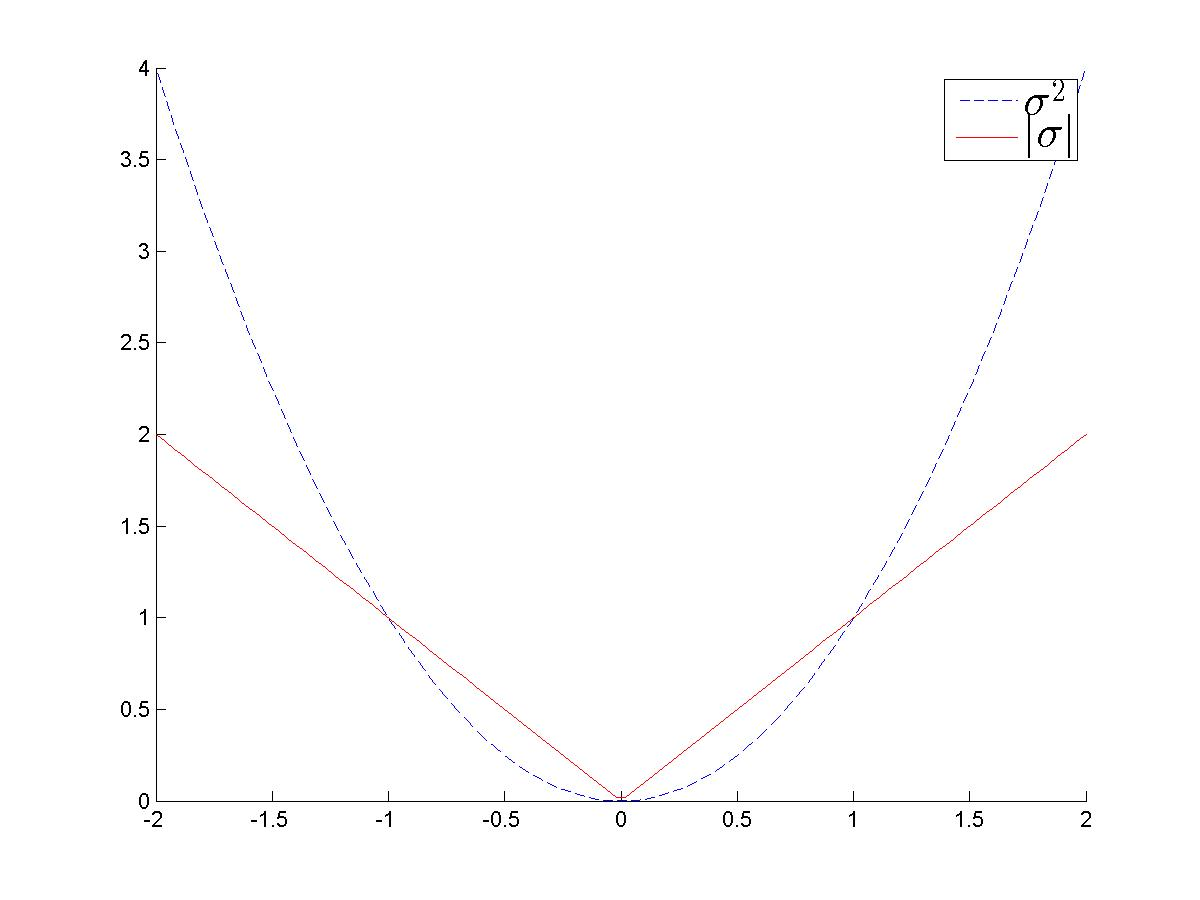
\includegraphics[width = 3in]{img/func} 
	\caption{  throw off of $L^1$ vs $L^2$ function }
\end{figure}


\section{Improvements}
\subsection{Low Pass Filter}

As stated above, most of the algorithms use a coarse to fine estimation, and, for each level, an iterative approximation is performed.
One of the downside of this approach is that if any outliers are present in the for at a lower level, this error will be propagated to all finer levels up to the final result, damaging the overall outcome of the algorithm.

In the papers comparing some of the existing algorithms, the implementations take a median filter somewhere in the algorithm.

In \cite{fleet2006}, the problem of aliasing is considered for bigger displacements, in the sampling procedure. The authors solve this problem by applying a blurring filer over the images, before computing the gradients of the images. From this they apply estimate the velocities for each level.

Also, in \cite{sun2010}, by analysing the best practices in solving the optical flow problem, it is proven that, if a median filter applied after each warp, the robustness and the accuracy of the algorithms is increased.
The robustness is a weak point of the differential methods. Outliers can completely throw off the energy function, especially in $L^2$ methods.
Their results compare different sizes of the median filter, and no filer of different algorithms. The best results are obtained with a $5 \times 5$ kernel. Also the accuracy of the results when no filter was applied is significantly lower.  


\subsection{Cross Correlation}
The cross correlation function measures the similarity between 2 signals.
The normalized cross correlation takes values in $[0,1]$, where $1$ is a total match between the signals and $0$ is a total mismatch between them.

In \cite{drulea2013}, the classical sum of squared difference, the data term is expressed as a zero normal cross correlation, this being more discriminative. 
 
 \begin{equation}
 C(i) = \frac{I(s)- \mu(i)}{\sigma(i)}
 \end{equation}
As shown above, each point of the image, if passed trough a cross correlation transom, from which results a matrix of the same size as the neighbourhood considered. to find the minimum, the data term is further expanded with classic differential methods it is added the smoothness term.

\subsection{Bilateral Filter} \label{bf}
The bilateral filter is a smoothing filter, but the accuracy along edges is kept. 
As proposed in \cite{tomasi1998bilateral}, the filter has two elements. The geometric distance, from the classical lowpass filter, let's take Gaussian for example. Each neighbour pixel will influence the output proportionally with its distance to the current pixel. On the other hand, the chromatic component measures the photochromacy between the neighbours and the central pixel. This can be expressed as the difference between the intensity of the neighbour pixel and the centre. 

In the Gaussian case, one could get the normalization term, which is
\begin{equation} \label{bilateralFilterTerm}
	e^{-\big(\ \frac{\Delta_c(i,s)}{2\sigma_c^2}+ \frac{\Delta_d(i,s)}{2\sigma_d^2}\big)}
\end{equation}

This normalization term can measure the likelihood of being on the edge of a pixel. An exaple of the bilateral filter transform is given in \ref{BFexaple}. It can be observed in the left figure, \ref{bfb}, the brighter areas on the planes of the object indicate a value near to $1$, and the darker areas, indicating $0$ are present on the edges of the objects.

\begin{figure} \label{BFexaple}
	\subfloat[]{\label{bfa}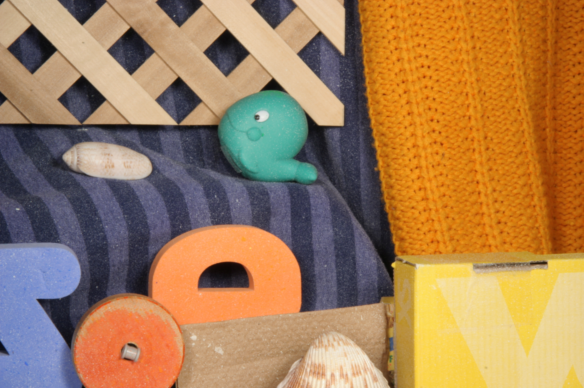
\includegraphics[width = 3in]{img/frame10}} 
	\subfloat[]{\label{bfb}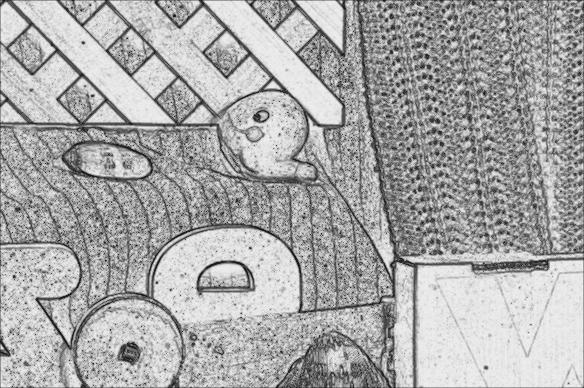
\includegraphics[width = 3in]{img/bf}}
	\caption{Example of the bilateral filter transform. \ref{bfa} is the original image, on which the formula \ref{bilateralFilterTerm} was applied. The result is shown on the right in \ref{bfb}}
\end{figure}

In \cite{drulea2013}, this formulation of the bilateral filter is used as a component of smoothness term. The smoothness constraint says that, the velocity of the neighbour pixels is the same. This applies, of course only if the neighbour pixels belong to the same object. The classic methods based on the smoothness constraint have large errors along the edges. By considering the bilateral filter term \ref{bilateralFilterTerm}, one can easily reduce the smoothness penalty for velocities that do not belong to the same object, by simply applying the dot product between the bilateral filter term and the first norm of the difference. 

\subsection{Census transform}

In Census transform, the intensities of pixels are mapped in a string of bits. The string is formed based on the relation of the current pixel to its neighbours.  Considering a $3\times3$ window, the centre is compared with its neighbours after the function:

\begin{equation} \label{censtr}
	\mathcal{C}(x,x') =
	\left\{
	\begin{array}{ll}
	1  & \mbox{if } I(x) - I(x') > th \\
	1  & \mbox{if } |I(x) - I(x')| \leq th  \\
	-x & \mbox{if } I(x) - I(x') <- th 
	\end{array}
	\right.
\end{equation}
where $I(x)$ is the intensity of the pixel $x$ and $x'$ is the neighbour. After the neighbour matrix was transformed, it is unwrapped, usually from the upper left corner, clockwise. Let us take an example. In figure \ref{cens}, the Census transform is applied \ref{censtr}, with a threshold of 10.

\begin{figure} \label{cens}
	\centering
	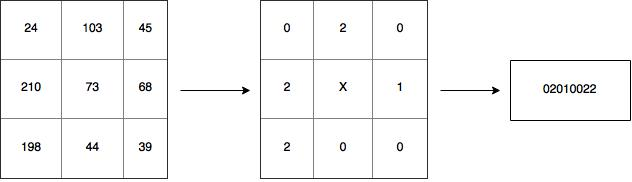
\includegraphics[width = 5in]{img/cens} 
	\caption{ Census Transform example to signature vector }
\end{figure}


There must be a balance when choosing the threshold, between a value that is to high and causes insensitivity to light chances and a value that is too small where the uniqueness of the signature bit is affected.

The transform is applied on each pixel of a image. The image will be described by a series of signature vectors. Each of this vectors are stored in a Hash-Table together with their coordinates.
Then the second image is transformed too. A matching is done between the signatures of the second image and the signatures in the table, resulting in a list of possible correspondences for each entry or a null if the signature has no match. In case of multiple match, the pixels' intensities are compared or, if there is still no unique solution, the closest match, distance wise, is taken.


An advantage of this solution is that the algorithm can detect large displacements, like objects jumping from one side to another of the image, unlike classic differential methods. 

Due to the nature of the algorithm, it can be implemented on parallel hardware, like FPGAs, allowing for real-time computation. 


But because of the transform, and the threshold, ignoring pixels with low variance, there is important loss in accuracy.


\chapter{Analysis and Theoretical Foundation of existing algorithms}
\label{ch:analysis}

There are different approaches in computing the optical flow. From the fundamental methods, the field of study advanced tremendously in terms of speed and accuracy of solving the problem. Although highly improved results, the newer approaches are based on the same assumptions and start from the same point as the original formulation of Horn and Schunch, and Lucas and Kanade. 

Although this algorithms are quite different, one being global formulation and the other a local one, modern approaches apply principles from both. The brightness consistency assumption is a good start point for many approaches, but it might be formulated in different form. Some algorithms use the Lukas Kanade approach style for a region based detection or feature tracking algorithms.




\section{Differential Methods}
The Horn and Schunk's solution is the basis of modern differential approaches. The optical flow is formulated as a equation that must be minimized.

To avoid the aperture problem, the equation is formulated from two constraints. Originally, the brightness constraint and the smoothness constraint. In most algorithms from this category the brightness constraint is kept and the second constraint is modified.
\subsection{The Brightness Constraint} \label{BrightnessConstr}

The brightness constraint requires a Lambertian surface (ideally mate), is valid only under constant lightening, the main illumination source should be at such a distance that it will not change the brightness of the objects. Also secondary illumination should not exist, so no inter-object reflection can appear.

 Also, a small motion is assumed from one frame to the next. 
 
Although all its  requirements which are almost never respected, at least not entirely, in real world, the brightness assumption has proven it's efficiency in may algorithms, being considered a good start point.

The brightness constraint assumes that the moving pixels of an image do not change their intensity in an image in time.


\begin{equation}  \label{Idt0}
\frac{\partial I}{\partial t} = 0
\end{equation}
From this, using multi-dimensional Euler-Lagrange equations (see appendix B for full demonstration), we obtain
\begin{equation} \label{Idt0_lagr}
\frac{\partial I}{\partial x}\frac{dx}{dt} +
\frac{\partial I}{\partial y}\frac{dy}{dt} +
\frac{\partial I}{\partial t} = 0
\end{equation}
The optical flow is given by the $x$ and $y$ derivative in time. Considering this, let
\begin{equation}
u = \frac{dx}{dt} \ \ \ , \ \ \  v = \frac{dy}{dt} \ \ \ and \ \ \ \nabla I=\begin{bmatrix}
I_x & I_y
\end{bmatrix} ^T
\end{equation} 
be the optical flow, $\boldsymbol{v}$ components. Denoting the temporal derivative with $I_t$, we obtain the gradient constraint. 
\begin{equation}
	\nabla I \cdot \boldsymbol{v}+I_t = 0
\end{equation}


\subsection{The Aperture Problem}
As a analogy, in motion perception, each retinal neuron captures only a small part of the visual field. This can be associated with seeing motion trough a small window, aperture. Because of the lack of context, uncertainty in speed, direction might appear. This uncertainty is called the aperture problem.
The brain solves this ambiguity by composing a big picture from each neuron's perception, transforms a local problem in a global one, meaning that each computed velocity depends on the entire image.
 
 
As in our seeing mechanism, in optical flow detection, when a solution is computed locally, a uncertainty of the motion arises. Of course, it is more likely to have bigger uncertainties in special cases. 

For example when there is no texture on the objects. As shown in figure \ref{apertureimg}, let the rectangle be the aperture, and the motion be given by the line moving from left to right. Let us consider the bolted point. the viewer can only say with certainty that the bolted dot will move from left to right, having no information about the movement on vertical, not the speed of the dot. The line can move either pure horizontally, slightly up, or slightly down. It is only when the viewer takes in account the end points of the line, he can state that the line is moving slightly up.  

\begin{figure}
	\label{apertureimg}
	\centering
	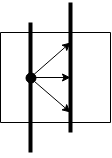
\includegraphics{img/Aperture}
	\caption{Example of aperture problem by the movement of a line.}
\end{figure}

On the other hand, if the texture is to structured, it may also bring uncertainty to the solution. If we take for example a sinusoidal wave like in \ref{apertureimgSin}, there is no telling if the signal moves up or down. As states in \cite{barron1994}, the authors encounter problems when testing the solutions based on SSD on such input sequences. Because of the periodical signal, the algorithms found more than one solution. As they made the search window bigger, the more (ghost as they called it) local minimas the algorithm found. 

\begin{figure}
	\label{apertureimgSin}
	\centering
	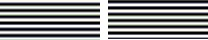
\includegraphics{img/sin}
	\caption{Example of aperture problem by the movement of a sinusoidal signal.}
\end{figure}


In optical flow, the simplest solution is the brightness assumption, that neighbouring pixels have the same movement.

\subsection{Lucas-Kanade}
Lucas-Kanade method solves the flow as a feature tracking algorithm. This differential method takes in account only the neighbourhood, solving for each pixel with last square estimation. From the brightness assumption, for a neighbourhood $\Omega$, the flow vector $[u_i,v_i]$ must satisfy: 
\begin{equation}
\begin{split}
	&I_x(x_1)+I_y(x_1) = - I_t	\\
	&I_x(x_2)+I_y(x_2) = - I_t \\
	&\vdots \\
	&I_x(x_n)+I_y(x_n) = - I_t 
	\end{split}
\end{equation} 

where $x_1$, $x_1$,  $...$,  $x_n$ are in the neighbourhood of pixel $i$.

Using the least square method, for each pixel in the image the energy function can be stated as:
\begin{equation} \label{gradientSumN}
	E(x) = \sum_{\substack{x \in \Omega}}
	 W^2(x)[\nabla I(x)\cdot \boldsymbol{v}+I_t(x)]^2
\end{equation}
where $W$ is a window function, Gaussian like, giving more weight to the canter pixel, rather than the neighbours.

To minimize $E(x)$, variational calculus is applied, and the derivatives of the equation \ref{gradientSumN} with respect to $u$ an $v$, respectively will be 0.

\begin{equation}
	\begin{split}
	\frac{\partial E}{\partial u} =  \sum_{\substack{x \in \Omega}}
	W^2(x)[I_x^2 u + I_x I_y v + I_x I_t] = 0 \\ 
	\frac{\partial E}{\partial v} =  \sum_{\substack{x \in \Omega}}
	W^2(x)[ I_x I_y u + I_y^2 v + I_y I_t]  = 0
	\end{split}
\end{equation}

If we demote
\begin{equation}
\begin{split}
A = \begin{bmatrix}
\nabla I(x_1), \ \dots , \ \nabla I(x_n)
\end{bmatrix} ^T \\
W = diag
\begin{bmatrix}
W(x_1), \ \dots , \ W(x_n)
\end{bmatrix}
\\
b = 
\begin{bmatrix}
-I_t(x_1), \ \dots, \ -I_t(x_n) 
\end{bmatrix}
\end{split}
\end{equation}
for each $n$ points $x_i \in \Omega$. Then, to minimize equation \ref{gradientSumN}, we differentiate  and the solution will be given by,
\begin{equation}
	A^T W^2 A  \boldsymbol{v} = A^T W^2 b 
\end{equation}
We multiplied the equation with $A^T$ on the left hand side, make the matrix nonsingular and be able to compute it's inverse. The Flow vector will be equal with:
\begin{equation}
\boldsymbol{v} = [A^T W^2 A  ]^{-1}A^T W^2 b
\end{equation}
where,

\begin{equation}
A^T W^2 A = 
\begin{bmatrix}
\sum W^2(x)I_x^2(x) \ \ \  
&\sum W^2(x)I_x(x) I_y(x) \\
\sum W^2(x)I_x(x) I_y(x) \ \ \  
&\sum W^2(x)I_y^2(x) 
\end{bmatrix}
\end{equation}
and
\begin{equation}
A^T W^2 b = 
\begin{bmatrix}
-\sum W^2(x)I_x(x)I_t(x)   \\
-\sum W^2(x)I_y(x) I_t(x)  

\end{bmatrix}
\end{equation}
 
by simple calculations we obtain
\begin{equation}
\begin{split}
	u =\frac{-\sum W^2I_y^2\ \sum W^2I_xI_t 
		+ \sum W^2I_x I_y  \sum W^2I_yI_t }
	{\sum W^2 I_x^2 \sum W^2 I_y^2
		- (\sum W^2 I_x I_y)^2 } \\
	u =\frac{\sum W^2I_x I_t\ \sum W^2I_xI_y 
		 - \sum W^2I_x^2  \sum W^2I_yI_t }
	{\sum W^2 I_x^2 \sum W^2 I_y^2
		- (\sum W^2 I_x I_y)^2 } \\
\end{split}
\end{equation}

\subsection{Correcting term}
As in the Lucas Kanade method, the flow equation can be solved, neglecting the aperture problem, as a local solution. But, as the window is getting bigger, the flow vector will be influenced by more neighbours, and the aperture problem is felt more as the results are more noisy. Why would one try to enlarge the system of equations? Well, because put it in a context and everything can change. By connecting the pixels with their neighbours, all te pieces will be connected and the system can be viewed as an ensemble. The results get better by solving the aperture problems. 


For example, as stated before, on surfaces with smooth, or no texture, the flow cannot be computed with a local method. But, if for a pixel in a textureless area, the flow is computed taking in account its neighbours, flow information will be propagated to it. In image \ref{HSExamplep}, it is shown the flow output for a square moving right and upwards. it can be sen the propagation of the flow between iterations 3 and 100.

\begin{figure} \label{HSExamplep}
	\centering
	\subfloat[]{\label{hspa}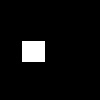
\includegraphics[width = 2in]{img/1}} 
	\subfloat[]{\label{hspb}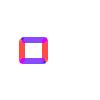
\includegraphics[width = 2in]{img/firsto}}
	\subfloat[]{\label{hspc}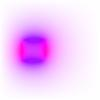
\includegraphics[width = 2in]{img/firsto1}}
	\caption{In \ref{hspa} is the square on which the propagation was tested. in \ref{hspb} and \ref{hspc} , example of flow propagation from iteration 3 to 100}
\end{figure}

In addition to the brightness constraint, Horn and Schunk take a second term in equation, the smoothness constraint. The value of a pixel will be probably very close to its neighbours. It is probably the simplest regularizator. 





\begin{equation} \label{smoothEq}
	E_{smooth} = \iint (\left\Vert\nabla u \right\Vert_2^2 +\left\Vert\nabla v \right\Vert_2^2)dxdy
\end{equation}
where
\begin{equation} \label{mynabla}
	\nabla = \frac{\partial^2}{\partial x^2} + \frac{\partial^2}{\partial y^2}
\end{equation}
which means if the flow differs from a pixel to another (on $x$ and $y$ directions), the smoothness equation, \ref{smoothEq} will be high. As the algorithm tries to minimize the energy function\ref{HSEq}, the second term, \ref{smoothEq}, will also be minimized. If this term is closer to zero, the flow derivatives over $x$ and $y$  are smaller, which means the difference with the  neighbours is also smaller, in other words the flow is smooth.

Nagel, in \cite{nagel1983constraints} proposes another smoothing term, in which he introduces also the gradient. It is based on the idea that errors often occur over the edges and the gradient has its greatest value on the edges. As it takes the gradient with the flow, the term is anisotropic. 

\begin{equation}
	\frac{\alpha^2}{\Arrowvert \nabla I\Arrowvert_2^2 \delta}[(u_xI_y- u_y I_x)^2+ (v_xI_y- v_y I_x)^2+ \delta(u_x^2+ u_y^2+v_x^2+ v_y^2)]
\end{equation}
 

The smooth term is more or less taken in account, depending on the nature of the input sequence. On some it works better with a higher weight, or in some, lower. Probably the best approach is to vary $\lambda$ weight of the second term in the flow equation \ref{HSEq}, and compare the results, like in a training stage of the program. Usually $\lambda$ is less than $1$ to avoid over smoothing.
\begin{equation}
	E = E_{data}+\lambda E_{smooth}
\end{equation}

To avoid this overall smoothing, as pixels may not be acting as a whole, $\lambda$ could be a matrix instead of a term, so each pixel can be influenced in his own percent of the neighbours.
An solution in computing this weight can be taken form the bilateral filter. The weight can be computed as explained in
\ref{bf}, so the smoothing term will influence each pixel differently. As when the pixel is on the edge, there should not be any influence from the neighbours, otherwise resulting in noisy results on the edges; but when the pixel is in the middle of an object, the velocity should be influenced by its neighbours.

\section{Coarse-to-fine}
Differential methods cannot approximate large displacements. This is due to the small motion assumption from the data term.
The data term is expanded with Euler-Lagrange equation and then expressed as a sum of partial derivatives. To discretize this derivatives a small step is necessary, usually of one pixel. This further means that motion larger than the with of the derivative window will not be detected. Also the kernel cannot be wider than one pixel on each side, because the small step requirement of the derivative.


This problem can be solved with coarse-to-fine method.
For example, in the original Horn Schunk formulation, the algorithm contains no Coarse to fine strategy. But, when this approach is added to the implementation the error of the results drop significantly. As it can be seen in the images in \ref{HSExample} When the flow is computed with the Coarse-to-fine approach the result are better. for this example in particular, the mean angular error without the pyramidal approach is $30.86$ and after is decreased to $15.94$





\begin{figure} \label{HSExample}
	\subfloat[]{\label{hsa}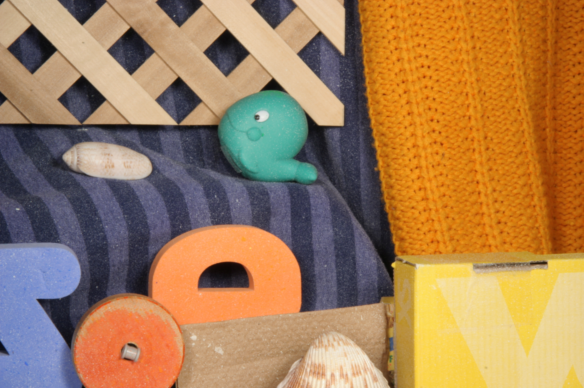
\includegraphics[width = 3in]{img/frame10}} 
	\subfloat[]{\label{hsb}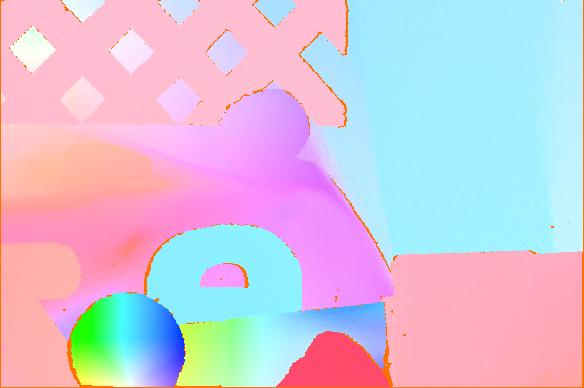
\includegraphics[width = 3in]{img/realflow}}\\
	\subfloat[]{\label{hsc}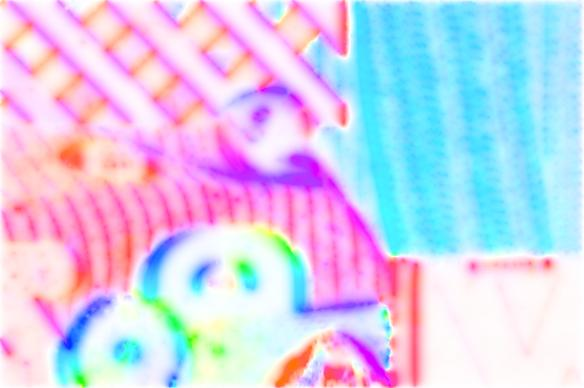
\includegraphics[width = 3in]{img/HS}}
	\subfloat[]{\label{hsd}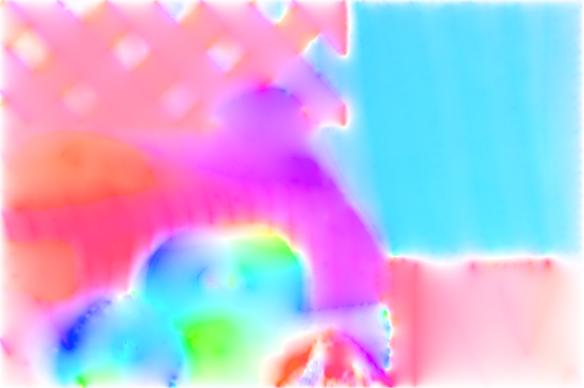
\includegraphics[width = 3in]{img/HSPyr}} 
	\caption{Example of the improvement the coarse to fine approach gives an algorithm. In picture \ref{hsa} is one of the 2 images of the sequence on which the flow is to be computed. In \ref{hsb} is the flow according to Middlebury. In \ref{hsc} is the flow computed with classical Horn and Schunk algorithm. And in \ref{hsd} is the same algorithm which was encapsulated in a coarse to fine strategy.}
\end{figure}

 
Firstly, Gaussian Pyramids are built by successively blurring and unsampling into images of smaller and smaller resolutions. The unsampeling is done until the smallest resolution is about 30 pixels width or height.  Then, the flow is iteratively computed between each level of the pyramid, from the corest to the finest.
\subsection{Gaussian Pyramids}
The pyramid of an image is a multi-scale representation of it. In order to obtain the pyramids, successive smoothing and subsampling techniques are applied.  Each level is computed from the previous, recursively.

\begin{figure}
	\label{PyrGr}
	\centering
	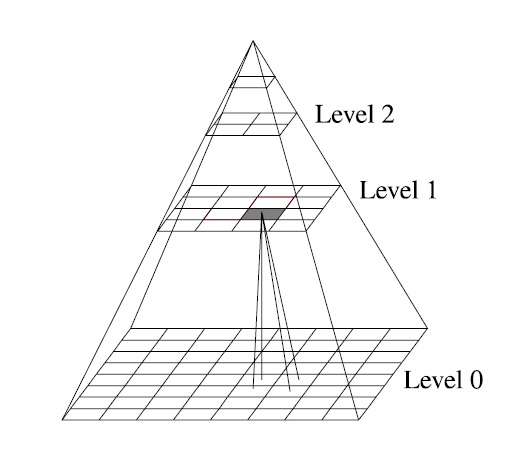
\includegraphics[width = 4in]{img/pyrLvls}
	\caption{visual representation of a pyramid. Taken from \cite{wedel2011stereo}}
\end{figure}



\paragraph{Building The pyramid} 
 Let us consider an image $I$ of size $m \times n$. The first level of the pyramid, the base is the image, $I_0$ is the image $I$, itself. The next level, $I_1$, is computed from $I_0$. The image $I_0$ is convoluted with a Gauss kernel, than the filtered image is sampled. $I_1$ is obtained with the dimensions $(m_0/sampling factor \times n_0/samplig factor)$. 

Similarly, the next levels are obtained, the $I_2$ is computed from $I_1$, $I_3$ from $I_2$, and so on, as illustrated in picture.

Usually a sampling factor of $0.5$ is considered. If we consider $L$ the current level of the image, than we can obtain the $I_{L+1}$ image as fallows



\begin{equation} \label{eq1}
\begin{split}
I_{L+1}(x,y) = &\frac{1}{4}I_L(2x,2y)+\\
&\frac{1}{8}(I_L(2x-1,2y)+I_L(2x+1,2y)+I_L(2x,2y-1)+I_L(2x,2y+1))+\\
&\frac{1}{16}(I_L(2x-1,2y-1)+I_L(2x+1,2y+1)+I_L(2x-1,2y+1)+I_L(2x+1,2y-1) 
\end{split}
\end{equation}

The result of such computation is shown in figure \ref{cameraPyr}.

\begin{figure}
	\label{cameraPyr}
	\centering
	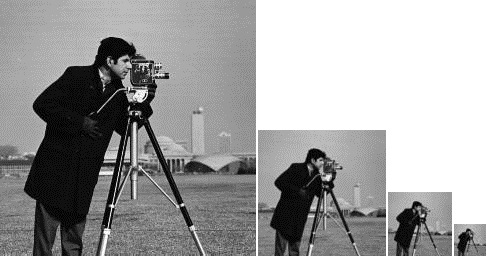
\includegraphics{img/cameraman}
	\caption{Example of a pyramid with 4 levels.}
\end{figure}


\paragraph{Choosing the pyramid height} 
Choosing the number of levels of aa pyramid depends of the nature of motion in the frame sequence and the downsampling factor.
 As stated in the chapter before \ref{pyrHeight}, the height of the pyramids is usually chosen to have around 20-30 pixels on the height of the image, or width, respectively. The height is given by
\begin{equation}
	pyramid_{height} = \frac{\log\left(\frac{p}{\min(ht,wt)}\right)}
							{\log(d)}
\end{equation}
where p is the number of pixels on the top level on the minimum between  width $wt$ or the height $ht$.
\subsection{Warping the flow on the image}


At new level of the pyramid, the second image is warped to the first.
The new computed flow is considered.
Let us consider the current level $l$, and the computed flow $\boldsymbol{v}_l$, on the next level $l+1$, the second image is warped with the $\boldsymbol{v}_l$ velocities from the previous level.
At a certain level $l+1$ the warped image is 
\begin{equation}
I_w = interpolation(I_l, w_l+dw)
\end{equation}
where $w_l$ is the flow computed until the level $l$ and $dw$ the  residual flow computed at level $l$. Some algorithms, like proximal point approximation, do not compute the residual flow, but update directly the new flow.

\section{$L^2$ Solutions}

First formulations were in the $L^2$ norm. For this simple approaches are used. As the function is convex and derivable, the solution is classic. First compute the partial derivatives, then equate them to 0. This are simple solutions, that run fast and don't consume to much memory. But this methods are very sensitive to noise. 

\subsection{Gauss-Seidel Iterations} \label{GaussSeidel}
Gauss Seidel is a iterative method for solving simultaneous equations. If we consider the system 
\begin{equation}
A\boldsymbol{x} = b
\end{equation}
where x is the unknown, the matrix $A$ can be decomposed in a sum of 2 matrices, the lower triangular and the upper.
\begin{equation}
	\begin{split}
	A &= L_* +U \\
	A &= \begin{bmatrix}
	a_{11} &  0  & \ldots & 0\\
	a_{21} &  a_{22} & \ldots & 0\\
	\vdots & \vdots & \ddots & \vdots\\
	a_{n1} &  a_{n2}       &\ldots & a_{nn}
	\end{bmatrix}  
	+  \begin{bmatrix}
	0 &  a_{12}  & \ldots & a_{1n}\\
	0 &  0 & \ldots &a_{2n}\\
	\vdots & \vdots & \ddots & \vdots\\
	0 &  0  &\ldots & 0
	\end{bmatrix} 
 	\end{split}
\end{equation}
	The equation becomes:
\begin{equation}
\begin{split}
	(L_*+U)\boldsymbol{x} = b\\
	L_*\boldsymbol{x}^{k+1} = b - U\boldsymbol{x}^{k}
\end{split}
\end{equation}
The algorithm takes a guess for the first step  $k$ of the iteration. The next steps are solved using the previous approximation and the solutions found up to the current point from the latest iteration. The algorithm stops when the solution converges, the iteration does not change the result significantly.

The Horn Schunk equation \ref{HSEq}, can be minimized using the Gauss Seidel Equations.
First, we need to derive by $u$  and $v$:
\begin{equation} \label{partialDer}
\begin{split} 
\frac{\partial E}{\partial u} = I_x(I_xu+I_yv+Iy) + \lambda(\bar{u}-u) \\
\frac{\partial E}{\partial v} = I_y(I_xu+I_yv+Iy) + \lambda(\bar{v}-v)
\end{split}
\end{equation}
Notice the substitution of the term $\nabla u ^2$ with $(\bar{u}-u)$, this is done like a Laplacian transform by unwrapping the $\nabla$ line in equation \ref{mynabla}.
 A matrix will be: 
$A_{2*i+1, 2*i+1} = I^2_{xi}+ \lambda$,
 $A_{2*i, 2*i} = I^2_{y}+ \lambda$,
$A_{2*i+1, 2*j} = I_{xi}I_{yi}$,  
$A_{2*i, 2*j+1} = I_{xi}I_{yi}$, 
 $A_{2*i+1, 2*j+1} = A_{2*i, 2*j} = \lambda$, where $j \in N_i $, by solving the equation for $\boldsymbol{x}$, we obtain the iterations:
 \begin{equation} \label{GSEq}
 \begin{split}
 u^{k+1}_i = \frac{1}{I_{xi}^2+I_{yi}^2+ \lambda}
					 (
					 (I_{yi}^2+\lambda)(\sum_{j \in \mathcal{N}_i;j<i} u_j^{k+1} + \sum_{j \in \mathcal{N}_i;j>i} u_j^k) \\
					 -I_{xi}I_{yi}(\sum_{j \in \mathcal{N}_i;j<i} v_j^{k+1} + \sum_{j \in \mathcal{N}_i;j>i} v_j^k)\\
					 -I_{xi}I_{ti}
					)
					 \\
   u^{k+1}_i = \frac{1}{I_{xi}^2+I_{yi}^2+ \lambda}
			   (
			   -I_{xi}I_{yi}(\sum_{j \in \mathcal{N}_i;j<i} u_j^{k+1} + \sum_{j \in \mathcal{N}_i;j>i} u_j^k)\\
			   +(I_{yi}^2+\lambda)(\sum_{j \in \mathcal{N}_i;j<i} v_j^{k+1} + \sum_{j \in \mathcal{N}_i;j<i} v_j^k)\\
			   -I_{yi}I_{ti}
			   )
 \end{split}
 \end{equation}
\subsection{Jacobi Iterations}
Like Gauss Seidel, the Jacobi method solves a system of linear equations. It is generally used when the system is diagonally dominant. 

If we consider the system 
\begin{equation}
	A\boldsymbol{x} = b
\end{equation}
where x is the unknown, the matrix $A$ can be decomposed in a sum of 2 matrices, the principal diagonal and the rest of the elements.

\begin{equation}
	\begin{split}
	A &= D + E \\
	A &= 
		\begin{bmatrix}
			a_{11} &  0  & \ldots & 0\\
				0	 &  a_{22} & \ldots & 0\\
			\vdots & \vdots & \ddots & \vdots\\
			0   &  0      &\ldots & a_{nn}
		\end{bmatrix}
		+
		\begin{bmatrix}
			0 &  a_{12}  & \ldots & a_{1n}\\
			a_{21} &  a_{22} & \ldots & a_{2n}\\
			\vdots & \vdots & \ddots & \vdots\\
			a_{n1} &  a_{n2}       &\ldots & 0
		\end{bmatrix}
	\end{split}
\end{equation}

The equation becomes:
\begin{equation}
\begin{split}
(D+E)\boldsymbol{x} = b\\
D\boldsymbol{x}^{k+1} = b - E\boldsymbol{x}^{k}
\end{split}
\end{equation}

The Jacobi iterations are used by Horn and Schunk in solving the minimization of the energy function. As can be observed, the method finds each $x$ from all it's previous guess but itself. Applied on Horn and Schunk's partial derivatives, the solution can be expressed as:

\begin{equation} \label{JEq}
\begin{split}
u^{k+1}_i = \frac{1}{I_{xi}^2+I_{yi}^2+ \lambda}
\left(
(I_{yi}^2+\lambda)(\sum_{j \in \mathcal{N}_i} u_j^{k})
-I_{xi}I_{yi}(\sum_{j \in \mathcal{N}_i} v_j^{k})
-I_{xi}I_{ti}
\right)
\\
u^{k+1}_i = \frac{1}{I_{xi}^2+I_{yi}^2+ \lambda}
\left(
-I_{xi}I_{yi}(\sum_{j \in \mathcal{N}_i} u_j^{k})
+(I_{yi}^2+\lambda)(\sum_{j \in \mathcal{N}_i} v_j^{k})
-I_{yi}I_{ti}
\right)
\end{split}
\end{equation}

Notice the difference between Gauss-Seidel and Jacobi method. The first one uses the solution for $x$ as soon as is available, while the Jacobi iterations relay only on the previous approximation.


The math between equation \ref{partialDer} and the iteration equations \ref{GSEq} and \ref{JEq} can be found in Appendix B \ref{GSDemo}.


\section{$L^1$ approach}

When the penalty function, $E(x)$ is of type $L^2$, like $\sigma^2(x)$,  the minimization problem is simple. One can reach the solution trough variational calculus, by differentiating the whole energy function with respect to $u$ and $v$, equalising with 0, and solving the system.  
For a higher robustness, current algorithms tend to use a $L^1$ penalty function, like modulus, others use a combination of both $L^2$ and $L^1$ penalty functions, for example, one for the data energy and one for the smoothness energy.

For this kind of formulations, the minimization can not be done any more trough differential techniques, and other approaches are used.

The smoothness term is the on that is more likely to give erroneous results, as the most outliers are present in the edge areas. Further will be presented two methods studied for solving thee $L^1$ norm. Both of the have only the correction term in $L^1$, the first remaining in $L^2$.

\subsection{Projected Proximal Point}


\subsection{Least Mixed Norm} \label{lmn}
The Least Mixed Norm (LMN) solution originates from the image restoration problems, belonging from the family of interior point algorithms. The objective is to minimize a $L^2-L^1$ function:
\begin{equation} \label{l2l1}
	\min_{\boldsymbol{f}}\Arrowvert g - H\boldsymbol{f}\Arrowvert_2^2+ \alpha\Arrowvert R \boldsymbol{f}\Arrowvert_1
\end{equation}

In \cite{fu2006efficient}, the problem is explained as a image restoration solution, but as the general function, \ref{l2l1}, matches the optical flow total energy function, this solution can be applied in the optical flow computation, considering $\boldsymbol{f}$ the pair of field vectors $(u,v)$.

Let us now discuss the solution presented in \cite{fu2006efficient}.

First le us write the data term, as a sun of it's positive and negative values:  $\alpha R \boldsymbol{f} = \boldsymbol{v}^+ + \boldsymbol{v}^-$, where $\boldsymbol{v}^+ = \max(\alpha R \boldsymbol{f}, 0) $, and  $\boldsymbol{v}^- = \max(-\alpha R \boldsymbol{f}, 0) $. Considering $\boldsymbol{1}$ a column of ones, the function becomes:

\begin{equation} \label{l2l1}
\min_{\boldsymbol{f}}\Arrowvert g - H\boldsymbol{f}\Arrowvert_2^2+ 
\boldsymbol{1}^T \boldsymbol{v}^+ +\boldsymbol{1}^T \boldsymbol{v}^-
\end{equation}
The function becomes:

\begin{equation}
	\min_{\boldsymbol{x}}\frac{1}{2}\boldsymbol{x}G\boldsymbol{x} + \boldsymbol{c}^T\boldsymbol{x} \ \ \
	\textnormal{ subject to } \ \ \  A\boldsymbol{x} = \boldsymbol{b}
\end{equation}

where
\begin{equation} \label{lmnBigM}
	\begin{split}
	G = \begin{bmatrix}
	2H^TH & 0 & 0\\
	 0 & 0 & 0 \\
	 0 & 0& 0
	\end{bmatrix} \ \ \ 
	A = \begin{bmatrix}
	\alpha R & -I & I
	\end{bmatrix} \\
	\boldsymbol{b} = \boldsymbol{0} , \ \ \ 
	 \boldsymbol{x} = \begin{bmatrix}
	 \boldsymbol{f} \\ \boldsymbol{v}^+
 \\\boldsymbol{v}^-
 	 \end{bmatrix} ,\ \ \ \textnormal{and} \ \ \ 
 	  \boldsymbol{c} = \begin{bmatrix}
 	  -2H^T\boldsymbol{g} \\ \boldsymbol{1}
 	  \\\boldsymbol{1}
 	  \end{bmatrix}
 	\end{split} 
\end{equation}
We can now write the Lagrange equation:

\begin{equation}
\mathcal{L}(\boldsymbol{x}, \boldsymbol{\lambda}, \boldsymbol{s}) = \frac{1}{2}\boldsymbol{x}G\boldsymbol{x} + \boldsymbol{c}^T\boldsymbol{x} - \boldsymbol{\lambda}^T(A\boldsymbol{x}-b) - \boldsymbol{s}^T
\boldsymbol{x}
\end{equation}
where $\lambda$ is the generalized Lagrange multiplier for the $A\boldsymbol{x} = \boldsymbol{b}$ constraint. Let $X$ and $S$ be sparse matrices with the diagonal elements from $\boldsymbol{x}$ and $\boldsymbol{s}$ unwrapped. The equation can be rewritten as:
\begin{equation}
F(\boldsymbol{x}, \boldsymbol{\lambda}, \boldsymbol{s}) = 
	\begin{bmatrix}
G\boldsymbol{x} + \boldsymbol{c}-A^T\boldsymbol{\lambda} - \boldsymbol{s}\\
A\boldsymbol{x}-\boldsymbol{b} \\
XS\boldsymbol{1}
	\end{bmatrix} = 0
\end{equation}
where the central path is
\begin{equation}
	F(\boldsymbol{x}_{\sigma\mu}, \boldsymbol{\lambda}_{\sigma\mu}, \boldsymbol{s}_{\sigma\mu}) = \begin{bmatrix}
	0 \\ 0 \\ \sigma\mu \boldsymbol{1}
	\end{bmatrix}
\end{equation}
where $\sigma \in (0,1)$ and $\mu$ is the arithmetic mean of $\boldsymbol{f}$. Rewriting using Newton step, the system becomes:

\begin{equation}
	\begin{bmatrix}
	G &-A^T & -I\\
	A & 0 & 0 \\
	S & 0  & X
	\end{bmatrix} 
	\begin{bmatrix}
	\Delta\boldsymbol{x} \\ \Delta\boldsymbol{\lambda} \\ \Delta\boldsymbol{s}
	\end{bmatrix} =
		\begin{bmatrix}
		\boldsymbol{-r_c} \\ \boldsymbol{-r_b} \\ \boldsymbol{-r_a}
		\end{bmatrix}
\end{equation}
where 
\begin{equation}
\boldsymbol{r}_c = G\boldsymbol{x} + \boldsymbol{c}-A^T\boldsymbol{\lambda} - \boldsymbol{s}, \ 
\boldsymbol{r}_b = A\boldsymbol{x}-\boldsymbol{b} \ \textnormal{and} \ 
\boldsymbol{r}_a = XS\boldsymbol{1}- \sigma\mu \boldsymbol{1}
\end{equation}
to reduce by $\Delta s$
\begin{equation}
	\begin{bmatrix}
	G+X^{-1}S &-A^T \\
	A & 0  
	\end{bmatrix} 
	\begin{bmatrix}
	\Delta\boldsymbol{x} \\ \Delta\boldsymbol{\lambda} 
	\end{bmatrix} =
	\begin{bmatrix}
	-\hat{\boldsymbol{r}}_c \\ \boldsymbol{-r_b} 
	\end{bmatrix}
\end{equation}
where $\hat{\boldsymbol{r}}_c = \boldsymbol{r}_c + X^{-1}\boldsymbol{r}_a$. Making the system symmetric:


\begin{equation}
\begin{bmatrix}
G+X^{-1}S &A^T \\
A & 0  
\end{bmatrix} 
\begin{bmatrix}
\Delta\boldsymbol{x} \\ -\Delta\boldsymbol{\lambda} 
\end{bmatrix} =
\begin{bmatrix}
-\hat{\boldsymbol{r}}_c \\ \boldsymbol{-r_b} 
\end{bmatrix}
\end{equation}

Let $D = S^{-1/2}X^{1/2}$, the let $D$ be decomposed in equal partitions over the diagonal. $D = diag(D_1, D_2, D_3)$ .
Then the system can be unwrapped as:
\begin{equation}
\begin{bmatrix}
2H^TH+D_1^{2} & 0 & 0 &\alpha R ^T\\
0 & D_2^{2} & 0 & 0 \\
 0 & 0 &  D_3^{2} & 0\\
\alpha R &-I & I & 0  
\end{bmatrix} 
\begin{bmatrix}
\Delta\boldsymbol{f} \\ 
\Delta\boldsymbol{v}^+ \\ 
\Delta\boldsymbol{v}^- \\ 
\Delta\boldsymbol{\lambda} 
\end{bmatrix} =
\begin{bmatrix}
-\hat{\boldsymbol{r}}_{c1} \\
-\hat{\boldsymbol{r}}_{c2} \\
-\hat{\boldsymbol{r}}_{c3} \\
 \boldsymbol{-r_b} 
\end{bmatrix}
\end{equation}
where $-\hat{\boldsymbol{r}}_c1$, $-\hat{\boldsymbol{r}}_c2$,  and $-\hat{\boldsymbol{r}}_c3$ are the appropriate vectors of $-\hat{\boldsymbol{r}}_c$, 
by removing $\Delta \boldsymbol{v}^+$ and $\Delta \boldsymbol{v}^-$ we obtain:

\begin{equation}
\begin{bmatrix}
2H^TH+D_1^{2} &\alpha R ^T\\
 \alpha R & -D_2^{2} + -D_3^{2} 
\end{bmatrix} 
\begin{bmatrix}
\Delta\boldsymbol{f} \\ 
\Delta\boldsymbol{\lambda} 
\end{bmatrix} =
\begin{bmatrix}
-\hat{\boldsymbol{r}}_{c1} \\
-\hat{\boldsymbol{r}}_b  
\end{bmatrix}
\end{equation}

 where 
 $-\hat{\boldsymbol{r}}_b =  \boldsymbol{-r_b} + D^2_2\hat{\boldsymbol{r}}_{c2} - D^2_3\hat{\boldsymbol{r}}_{c3}$
 and finally, eliminating $\Delta\boldsymbol{\lambda}$,
 \begin{equation} \label{lmnXeq}
 \begin{bmatrix}
 2H^TH+D_1^{-2} + \alpha R ^T( D_2^{2} +  D_3^{2} )^{-1}R
 \end{bmatrix} 
 \Delta\boldsymbol{f}  =
 -\tilde{\boldsymbol{r}}_{c1} \\
 \end{equation}
 where $\tilde{\boldsymbol{r}}_{c1} = \hat{\boldsymbol{r}}_{c1} + \alpha R ^T( D_2^{2} +  D_3^{2} )^{-1} \hat{\boldsymbol{r}}_{b}$
 
 The system will be solved for $\boldsymbol{f}$ with equation  \ref{lmnXeq}, and then the other unknowns can be computed:
 \begin{equation} \label{lmnReq}
 	\begin{split}
 	\boldsymbol{\lambda} = ( D_2^{2} +  D_3^{2} )^{-1}
 	(-\hat{\boldsymbol{r}}_{b} - \alpha R \boldsymbol{f})\\
 	\boldsymbol{v}^+ = D_2^{2}(-\hat{\boldsymbol{r}}_{c2} - \boldsymbol{\lambda})\\
	\boldsymbol{v}^- = D_3^{2}(-\hat{\boldsymbol{r}}_{c3} + \boldsymbol{\lambda})\\
 	\boldsymbol{s} =  G  \boldsymbol{x} -  A^T\boldsymbol{\lambda} + \boldsymbol{r}_c
 	\end{split}
 \end{equation}
 
 Now the system will be approximated iteratively. A initial guess is taken from the condition $A\boldsymbol{x} = b$ 




\section{Error Measurement}
Now that the problem is stated, in order to get an idea of which behaves better on what conditions, we can compare the flow results with a ground truth. Middlebury's website\cite{middleburry} proposes a challenging data sheet containing some of the top algorithms in optical flow, as they state in \cite{baker2011database}, by which they hope to encourage improvement. It \cite{middleburry} has a big database of the existing algorithms, classified by accuracy.
They have available a set of images on which the algorithms can be tested and measure their performance. Both realistic high speed camera and synthetic images can be downloaded from their database. For the artificially generated also the exact flow is available. This stands as a reference for the output of the algorithms. The error can be computed between this ground truth output and the result from the algorithms.

 Being referenced in most of the latest articles, it seems that this database is a good reference to modern approaches and their metrics.

\subsection{Cross correlation}

Cross correlation is a simple way to measure the difference between 2 signals. In image processing it is used as a normalized form. 

\begin{equation}
\frac{1}{n}\sum_{i,j} \frac{(f(i,j) - \bar{f})(f_{GT}(i,j) - \bar{f_{GT}})}{\sigma_f \sigma_{GT}}
\end{equation}


The results of this function will vary in $[0,1]$, $1$ meaning a total match and $0$ a total dismatch.
\subsection{Endpoint error}
For measuring this error, the length of the vectors is taken in account. This error is expressed as the sum of differences both on the $x$ and $y$ directions, stated in a $L^2$ or $L^1$ norm.

\begin{equation}
\begin{split}
\sum  \sqrt{(u-u_{gt})^2+(v-v_{gt})^2} \\ 
\sum |u-u_{gt}|+|v-v_{gt}|
\end{split}
\end{equation}

Although the endpoint error can provide useful information about the vector's length, it contains no measurement of  the vector's orientation. To obtain this, the angular measurement is used.
\subsection{Angular error}
As we are talking about vectors, we need a complementary measurements over the magnitude error presented above.


\begin{equation}
\sum  \arccos \left( \frac{u^T \cdot u_{gt}}{|u||u_{gt}|}\right)
\end{equation}
 This error measurement is frequently used, as it evaluates both the magnitude and the direction of the flow. Of course, it has its downsides. By taking the magnitude in equation, the higher speeds have a greater impact on the final result then the lower speeds having the same angular error. 

\chapter{Proposed algorithm}

Our solution starts from the optical flow formulation in \cite{drulea2013}.

\begin{equation} \label{druleaEq}
	E = \sum_{i \in \omega} \sum_{k}
	(C_t(i,k)+ \nabla C(i,k)\cdot(w_i-w_{0,i}))^2 + 
	\lambda
	\sum_k bf_{i,k} \cdot \Arrowvert w_k - w_i\Arrowvert_1
\end{equation}

To minimize this convex function, we will use the LMN method described in \ref{lmn},
To save computational time and memory, we compute directly the matrices from \ref{lmnBigM}.Finally the whole system will b determind by large sparse matrices. Let us take them one by on.

To compute $G$ we need $H^T H$, where $H$ the coefficient of the flow in the $L^2$ norm. From equation \ref{druleaEq}, with the flow  coefficient  $\nabla C(i,k)$ we get:
\begin{equation}
	H^TH = \begin{bmatrix}
	C_{x1}^2 & C_{x1} C_{y1} & 0 & 0 & \ldots & 0 & 0 \\
	 C_{x1} C_{y1} & C_{y1}^2 & 0 & 0 & \ldots & 0 & 0 \\
	 0 & 0 & C_{x2}^2 & C_{x2} C_{y2} & \ldots & 0 & 0 \\
	  0 & 0 &  C_{x2} C_{y2} & C_{y2}^2 & \ldots & 0  & 0\\
	  \vdots\\
	   0 & 0 &  0  & 0  & \ldots & C_{x\Omega}^2 & C_{x\Omega} C_{y\Omega} \\
	  	   0 & 0 &  0  & 0  & \ldots & C_{x\Omega} C_{y\Omega} & C_{y\Omega}^2\\
	\end{bmatrix}
\end{equation}

From this G matrix will be computed:
\begin{equation}
	G = \begin{bmatrix}
		2H^TH & 0 & 0\\
		0 & 0 & 0 \\
		0 & 0& 0
	\end{bmatrix}
\end{equation}

Regarding dimension, if $\Omega = m\times n$, is the image dimension, the matrix $H^TH$ will be $2\Omega \times 2 \Omega$ and G will be $6\Omega \times 6 \Omega$. It is important that all the matrices are sparse, and bended. 

Next, let us consider matrix $\boldsymbol{c}$; for this we need $H^T\boldsymbol{g}$. We now H, and ne notice the free term from \ref{druleaEq} Note $(C_{t1} - C_{xn}u_{old} - C_{yn}v_{old})$  with $e_n$. Then, $\boldsymbol{g}$ is:
$$
H^T \boldsymbol{g} = 
\begin{bmatrix}
& C_{x1}e_1 & 0 &\ldots & 0 & 0 \\ 
& 0 &  C_{y1}e1 &\ldots & 0  & 0\\
\vdots \\
& 0 & 0 &\ldots &  C_{x\Omega}e_{t\Omega}   & 0\\
& 0 & 0 &\ldots & 0 & C_{y\Omega}e_{t\Omega} 
\end{bmatrix}
$$

Now, to compute $A$ from the $L^1$ norm, we need $\alpha R$. We identify $\alpha$ as the $bf$ coefficient in \ref{druleaEq}
the  $\alpha$ will be:

\begin{equation}
 \alpha = \begin{bmatrix}
 &	bf_1  & 0  & 0  & 0  & \ldots & 0  & 0 \\
 &	0  & bf_1  & 0  & 0  & \ldots & 0  & 0 \\
 &			0  & 0  & bf_2  & 0  & \ldots & 0  & 0\\
 &				0  & 0  & 0  & bf_2  & \ldots & 0  & 0\\
 &				\vdots\\
& 			0 & 0  & 0  & 0  &\ldots & bf_\Omega  & 0 \\
& 				0  & 0  & 0  & 0  &\ldots & 0  & bf_\Omega\\
 \end{bmatrix}
\end{equation}
and $K$
\begin{equation}
K = \begin{bmatrix}
&	9  & 0  & 1  & 0  & 0  & 0  & \ldots & 0  & 0 \\
&	0  & 9  & 0  & 1  & 0  & 0  & \ldots & 0  & 0 \\
&	1  & 0  & 9  & 0  & 1  & 0  &\ldots & 0  & 0\\
&	0  & 1  & 0  & 9  & 0  & 1  &\ldots & 0  & 0\\
&	\vdots\\
& 	0 & 0  & 0  & 0  & 0  & 0  &\ldots &9  & 0 \\
& 	0  & 0  & 0  & 0  & 0  & 0  &\ldots & 0  & 9\\
\end{bmatrix}
\end{equation}
The $K$
 matrix has elements on the principal diagonal 9, on the diagonal shifted up and down it has groups of 6 ones and 2 zeros, on the diagonal shifted up and down with $2* column_{number}-2$ we have sequences of 2 zeros and 6 ones, on the diagonal shifted up and down with  $2* column_{number}$ we have full ones, and on $2* column_{number}+2$  shift we have groups of 6 ones and 2 zeros.
  
  A matrix will be defined as in \ref{lmnBigM}, with the size $2\Omega \times 6\Omega$
 
 Now that we have all the big matrices are determined, we can find the vector $\boldsymbol{x}$  and the other unknowns from equations \ref{lmnXeq} and \ref{lmnReq} .  
\chapter{Detailed Design and Implementation}


\section{Derivative discretization}

 For obtaining the derivatives of the image and also the gradient we used the discretized formula:
\begin{equation}
		\frac{\partial f(x, y)}{\partial x} =  \frac{f(x-h, y) - f(x+h,y)}{2h}
\end{equation}

By taking the small step $h = 1$ we can compute the derivatives and the gradient of the image.
For achieving this, the a Prewitt kernel convolution is used. The convolution process implies multiplying each pixel of a image and its neighbours by an kernel, chosen depending on the operation. Perwitt is one of the kernels used for derivatives along  Laplacian, Sobel and Roberts. The Perwitt filter is $\begin{bmatrix}-1 & 0 & 1\end{bmatrix}$ and  
$\begin{bmatrix}-1 & 0 & 1\end{bmatrix}^T$  for the horizontal axis, vertical respectively. It is relatively easy and inexpensive to compute. Generally it is used in the context of edge detection, but in our implementations, was used in the energy function, especially in the brightness constraint. 

When computing only the gradient, and the partial derivatives are not further used, the kernel applied is the Laplacian, also found in the context of edge detection. The general formula is:
\begin{equation}
f(x, y) =  \frac{f(x-h, y) + f(x+h,y) +f(x,y-h) +f(x+h,y) - 4f(x,y)}
{(2h)^2}
\end{equation}
 In \ref{GaussSeidel} when computing the derivative, the gradient $\nabla u$ was replaces with$\bar{u} - u)$. This is because the gradient was computed with a Laplace Kernel:
 \begin{equation}
 \frac{1}{9}
 \begin{bmatrix}
 	1 & 1 & 1 \\
 	1 & -9 & 1 \\
 	1 & 1 & 1
 \end{bmatrix}
 \end{equation}


Notice the property of the differentiative krnels, both Perwitt and Laplce, the sum of the elements must alwais be 0. 

\section{Sparse Matrix vs Iterative approach}

Sparse matrices are usually large matrices with most of the elements $0$. They are popular with solving large linear systems.

The memory advantage of sparse over full matrices is that in sparse only the non zero values and their indexes are stored. 

Computational wise it skips redundant operations with 0 such as addition and multiplication.

A special type of sparse are band matrices. This are regular sparse, the non-zero elements are grouped diagonally. This allows even more efficient memory use and computation time. 

\section{Downsamplig and Pyramidal Implementation}


\section{Output and MATLAB Colorspace}


For the flow output and visualization, the functions available on Middlebury ware used.
As their ground truth flow was encoded in .flo format, we kept the same convention. The .flo is the unwrapped flow matrix in a long stream. values are red one by one and then the flow is rearranged in a $m\times n \times 2$ matrix, where $m$ and $n$ are the flow field's height and width and 2, every vector's $x$ and $y$ components.

Middlebury\cite{middleburry} provides functions for writing and reading this files. 

For visualizing the output each vector is encoded to the MATLAB's colour space. As shown in \ref{colors}, the vectors on the write, expressed as arrows are encoded trough colour code. The colour notation is  used more that ht vector, because the changes in direction are more obvious. Also, the magnitude of the vector is encoded by the level of saturation of the colour, white representing no movement, and a full, saturated colour represents the widest movement of the flow. The pixel range between white and full colours vary, depending on the flow output. The function adapts this range to the needs. As can be observed, the encodings for the main directions are: indigo for up, red for right, yellow for down and cyan for left. On Middlebury's site, thy provide a function for the colour transform in the same package as the read and write functions mentioned earlier. They can be found on the datasets section as "flow-code".  

\begin{figure}
	\label{colors}
	\centering
	\subfloat{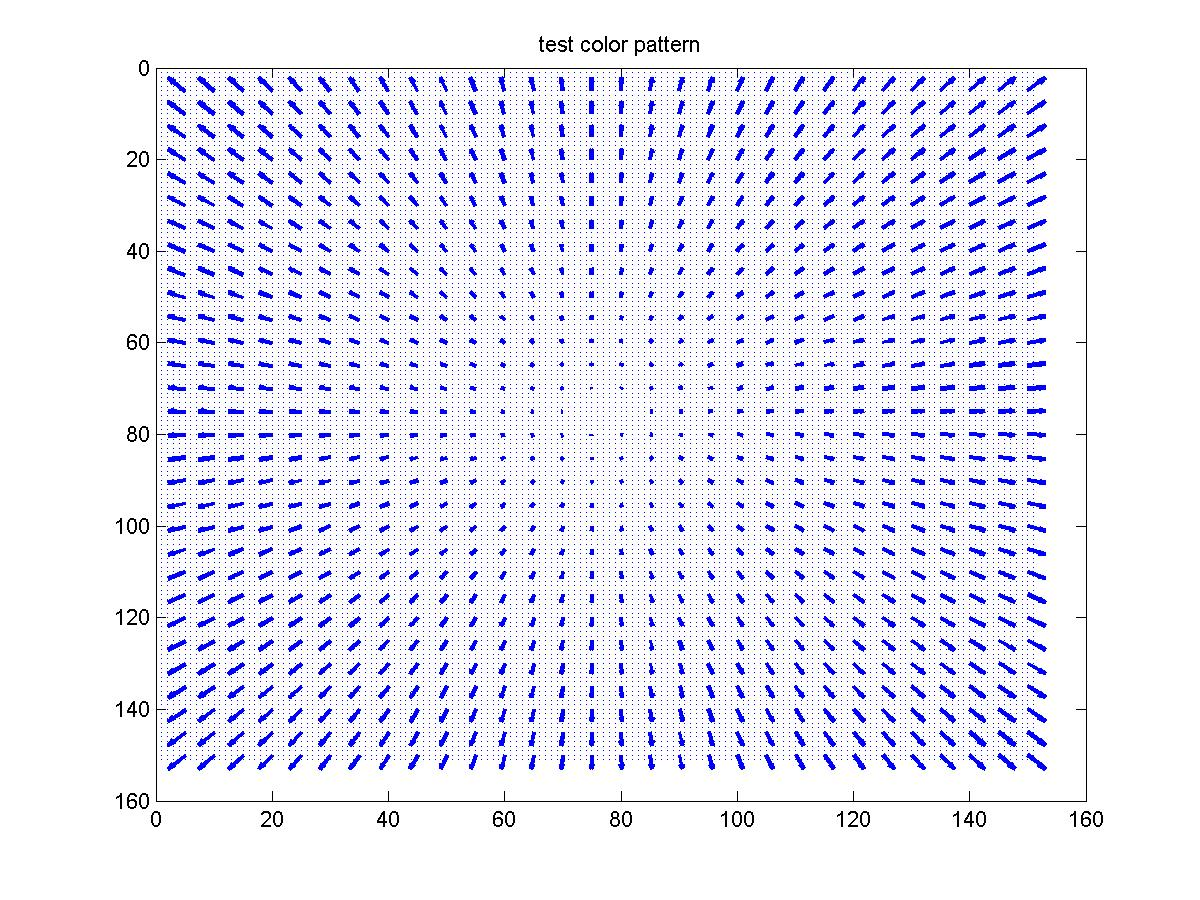
\includegraphics[width = 3in]{img/vectors}} 
	\subfloat{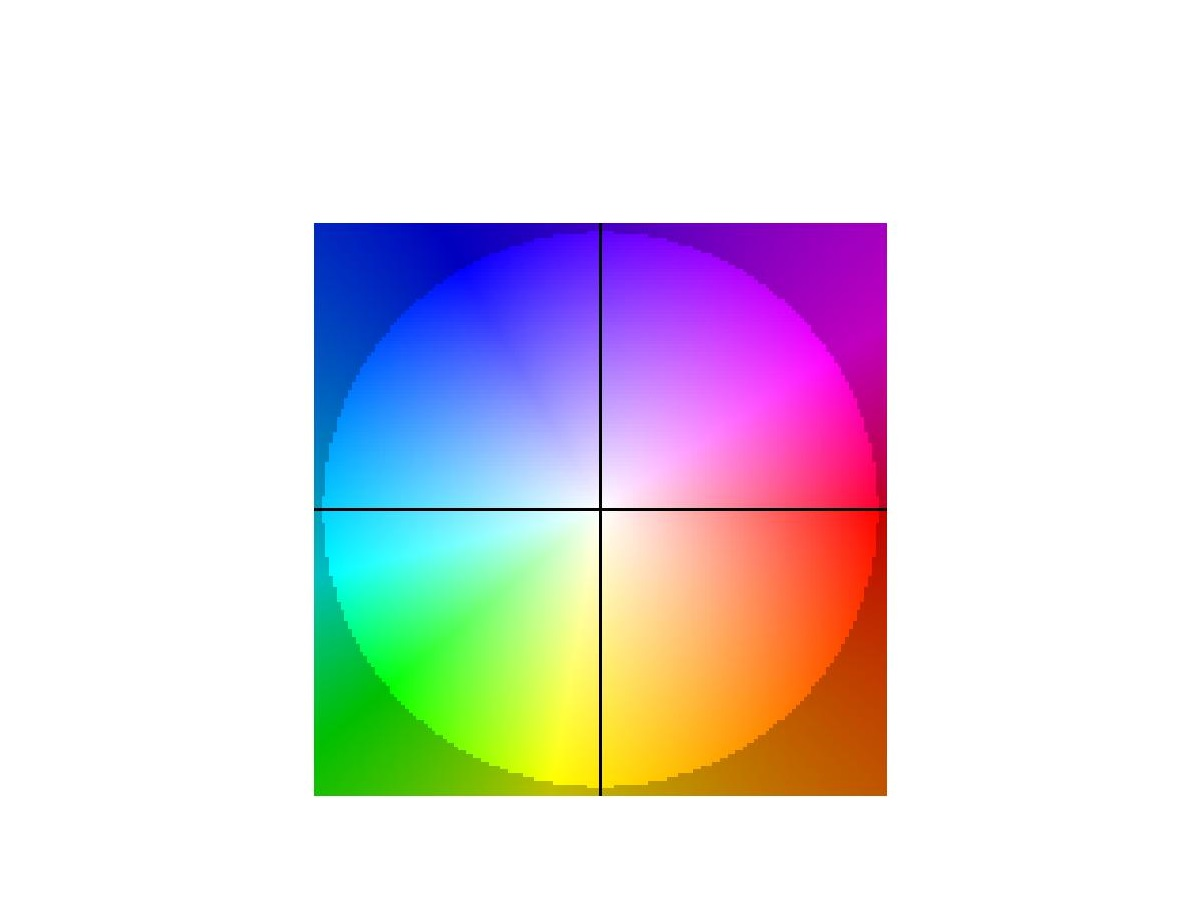
\includegraphics[width = 3.6in]{img/colors}} 
	\caption{Colour encoding.}
\end{figure}


\chapter{Testing and Validation}

About 5\% of the paper
\section{Title}
\section{Other title}

\chapter{User's manual}

In the installation description section your should detail the hardware and software resources needed for installing and running the application, and a step by step description of how your application can be deployed/installed. An administrator should be able to perform the installation/deployment based on your instructions.

In the user manual section you describe how to use the application from the point of view of a user with no inside technical information; this should be done with screen shots and a stepwize explanation of the interaction. Based on user's manual, a person should be able to use your product.

\section{Title}
\section{Other title}

\chapter{Conclusions}

About. 5\% of the whole

Here your write:
\begin{itemize}
\item a summary of your contributions/achievements,
\item a critical analysis of the achieved results,
\item a description of the possibilities of improving/further development.
\end{itemize}
\section{Title}
\section{Other title}


%\addcontentsline {toc}{chapter}{Bibliography} 
\bibliographystyle{IEEEtran} 
\bibliography{thesis}%same file name as for .bib

\appendix
\chapter{Relevant code}

\begin{verbatim}
Optimize (x,s,lambda)
\{
	D23SqInv = spdiags(1./ ...
				( ... 
					x(1+dim:2*dim)./s(1+dim:2*dim)+ ...
					x(1+2*dim:3*dim)./s(1+2*dim:3*dim)  ...
				) ...
				, 0, dim, dim);
	D23SqInv(isnan(D23SqInv)) = 0;
	
	D3 = spdiags(x(1:dim)./s(1:dim), 0, dim, dim);
	D2 = spdiags(x(1:dim)./s(1:dim), 0, dim, dim);
	D1Inv  = spdiags(s(1:dim)./x(1:dim), 0, dim, dim);        
	XInv = spdiags(1./x(:),0,3*dim, 3*dim);
	
	D3(isnan(D3)) = 0;
	D2(isnan(D2)) = 0;
	D1Inv(isnan(D1Inv)) = 0;
	XInv(isnan(XInv)) = 0;
	
	miu = mean(x(:).*s(:));
	sigma = std2(x(:).*s(:));
	ra = x(:).* s(:) - miu*sigma*ones(3*dim, 1);
	rc =  G*x+c-s-A'*l ;
	rb = A*x;
	rch =rc + XInv* ra;
	
	rch1 = rch(1:dim);
	rch2 = rch(1+dim:2*dim);
	rch3 = rch(1+2*dim:3*dim);
	
	rbh = rb + D2 * rch2 - D3 * rch3;
	rcTilda =rch1 +bfK'*(D23SqInv)*rbh;
	
	BigA = 2*G(1:dim, 1:dim)+D1Inv+bf2K'*D23SqInv*K;
	
	deltaF = gmres(BigA, -rcTilda);
	
	
	deltaL = D23SqInv*(-rbh-bfK*deltaF);
	deltaVp = D2*(-rch2-deltaL);
	deltaVm = D3*(-rch3-deltaL);
	deltaX = [deltaF; deltaVp; deltaVm];
	deltaS = G * deltaX- A'*deltaL+ rc;
	
	x = x + deltaX;
	s = s + deltaS;
	l = l + deltaL;
\}
\end{verbatim}

\chapter{Other relevant information (demonstrations, etc.)}
\section{Horn Scunk equation to Jacobi Iteration} \label{GSDemo}
First, let us define the staring equation.
\begin{equation}
	E = (I_xu+ I_yv + I_t)^2 + \lambda(\left\Vert(\nabla u) \right\Vert_2^2 +\left\Vert(\nabla v)\right\Vert_2^2)
\end{equation}
by discretizing $\left\Vert(\nabla u) \right\Vert_2^2$ with a Laplace filter, it can be rewritten as $(\bar{u}-u)^2$. The equation then becomes:
\begin{equation}
E = (I_xu+ I_yv + I_t)^2 + \lambda((\bar{u}-u)^2+(\bar{v}-v)^2)
\end{equation}
The we apply the partial derivatives and eqaual then to 0 in order to find the minimum, as E being convex,

\begin{equation} 
\begin{split} 
\frac{\partial E}{\partial u} = I_x(I_xu+I_yv+Iy) + \lambda(\bar{u}-u) \\
\frac{\partial E}{\partial v} = I_y(I_xu+I_yv+Iy) + \lambda(\bar{v}-v)
\end{split}
\end{equation}
Now to rearrange the  terms
\begin{equation} 
\begin{split} 
(I_x^2+\lambda)u + I_y I_x v  =  -I_xI_t + \lambda \bar{u} \\
I_y I_x u+(I_y^2+\lambda)v  = -I_yI_t + \lambda \bar{v} \\
\end{split}
\end{equation}
and in matrix form , $A \boldsymbol{x} = b$:

\begin{equation}
	\begin{bmatrix}
	I_x^2+\lambda & I_y I_x \\
	I_y I_x & (I_y^2+\lambda)
	\end{bmatrix}
	\cdot
	\begin{bmatrix}
	u \\
	v
	\end{bmatrix}
	=
		\begin{bmatrix}
	-I_xI_t + \lambda \bar{u}\\
	-I_yI_t + \lambda \bar{v}
		\end{bmatrix}
\end{equation}
The equation can be solved as $\boldsymbol{x} = A^{-1}b $. First to compute 
$A$'s determinant
\begin{equation}
	\frac{1}{\lambda(\lambda+I_x^2 + I_y^2)}
\end{equation}
the equation becomes:
\begin{equation}
\begin{bmatrix}
u \\
v
\end{bmatrix}
=
\frac{1}{\lambda(\lambda+I_x^2 + I_y^2)}
\begin{bmatrix}
I_y^2+\lambda & -I_y I_x \\
-I_y I_x & (I_x^2+\lambda)
\end{bmatrix}
\cdot
\begin{bmatrix}
-I_xI_t + \lambda \bar{u}\\
-I_yI_t + \lambda \bar{v}
\end{bmatrix}
\end{equation}

from this, on can easily find $u$ and $v$ as:
\begin{equation} \label{JEq}
\begin{split}
u^{k+1} = \frac{(I_{y}^2+\lambda)\bar{u}
	-I_{x}I_{y}\bar{v}
	-I_{x}I_{t}}{I_{x}^2+I_{y}^2+ \lambda}
\\
u^{k+1} = \frac{-I_{x}I_{y}\bar{u}
	+(I_{y}^2+\lambda)\bar{v}
	-I_{y}I_{t}}{I_{x}^2+I_{y}^2+ \lambda}
\end{split}
\end{equation}


\chapter{Published papers}

\end{document}
